%%%%%%%%%%%%%%%%%%%%%%%%%%%%%%%%%%%%%%%%%%%%%%%%%%%%%%%%%%%%%%%%%%%%%%%%%%%
%%%%%%%%%%%%%%%%%%%%%%%%%%%%%%%%%%%%%%%%%%%%%%%%%%%%%%%%%%%%%%%%%%%%%%%%%%%
%%% Inference rules for binary predicates
%%% Stephen J. Hegner
%%% Section 7
%%% 29 July 2021
%%%%%%%%%%%%%%%%%%%%%%%%%%%%%%%%%%%%%%%%%%%%%%%%%%%%%%%%%%%%%%%%%%%%%%%%%%%
%%%%%%%%%%%%%%%%%%%%%%%%%%%%%%%%%%%%%%%%%%%%%%%%%%%%%%%%%%%%%%%%%%%%%%%%%%%



 \section{Inference on Binary Rules Involving Negation}\label{sec:ninfrules}

     In this section, it is shown how to extend a sound and complete
proof system $\proofsys{A}$ for an Armstrong context $\armctxt{C}$ to
one which applies to all of $\allarm{\armctxt{C}}$.  It builds upon
the theoretical ideas developed in Sec.\ \ref{sec:negarm}, together
with the fundamental operation of \emph{swapping} to each rule in
$\proofsys{A}$, in which the conclusion of a rule is swapped with a
premise, and each negated.  It is shown that augmenting $\proofsys{A}$
with the set of all such swapped rules results in a sound and complete
inference system for $\allarm{\armctxt{C}}$.


 \begin{metalabpara}{context}{}
     {Context}\envlabel{ctxt:armctxtii}
 Throughout this section, unless stated specifically to the contrary,
$\proofsys{A}$\/ will be taken to be a sound but not necessarily
complete inference system for $\armctxt{C}$.  Note that the context
introduced in \envref{ctxt:armctxt} continues to hold.
    \par
    As in the previous section, the reader who is not interested in
the general case may fix $\armctxt{C}$ to be $\pbinconstrgrsch{G}$.
 \end{metalabpara}
    \parvert

    While the following result is straightforward, it is recorded
formally because it provides the key connection between the results of
Sec.\ \ref{sec:negarm} and the type of proof system developed in this
section.


 \begin{metaemphlabpara}{proposition}{Proposition}
    {Satisfiable inference in the Armstrong setting}\envlabel{prop:infarm}
     Let $\Phi$ be a satisfiable subset of $\armctxt{C}$, and let
 $\beta \in \armctxt{C}$ also be satisfiable.
    Assume furthermore that $\proofsys{A}$ complete.
   \baxblke
    \axitem{(a)} $\Phi \sentails \beta$ holds iff
   $\posof{\Phi} \syntailss[\proofsys{A}] \beta$.
    \axitem{(b)} $\Phi \sentails \mlnot\beta$ holds
  iff either
    $\posof{\Phi} \union \setbr{\beta} \syntailss[\proofsys{A}]
                                             \false$
 or else there is a
  $\mlnot\varphi \in \negof{\Phi}$ for which
    $\posof{\Phi} \union \setbr{\beta}
           \syntailss[\proofsys{A}] \varphi$.
   \eaxblk
 \begin{proof}
   The proof follows immediately from \envref{prop:entarm} and the
fact that $\proofsys{A}$\/ is sound and complete for $\armctxt{C}$.
 \end{proof}
 \end{metaemphlabpara}


 \begin{metalabpara}{mydefinition}{}
     {Swapping and swap closure}\envlabel{def:ruleswap}
     Let $\proofsys{A}$\, be an inference system for $\armctxt{C}$.
     Say that a rule $r \in \infrulesof{\proofsys{A}}$
\emph{has nonempty antecedent set} if
 $\antecedentsof{r} \neq \emptyset$.
     \par
     Let $r \in \infrulesof{\proofsys{A}}$ have nonempty
antecedent set
 $\antecedentsof{r} = \setdef{\alpha_i}{i \in \ccinterval{1}{k}}$
 and $\consequentof{r} = \setbr{\beta}$.
     The \emph{$\alpha_i$-swap} of $r$, denoted $\rswap{r}{\alpha_i}$,
is the rule obtained by replacing $\alpha_i$ with $\mlnot\beta$ as an
antecedent, and replacing $\beta$ with $\mlnot\alpha_i$ as the
consequent.  Visually, the transformation is
  \def\transto#1{\hspace*{#1} &\rightsquigarrow \hspace*{#1}}
  \def\sepval{0.5cm}
    \begin{align*}
    \tag{\ref{def:ruleswap}-1}
    \begin{prooftreem}
     \hypoi{\alpha_1~\alpha_2~\ldots~\alpha_{i-1}~\alpha_i~\alpha_{i+1}~
                      \ldots~\alpha_{k-1}~\alpha_k}
     \inferi{\beta}
    \end{prooftreem}
     \transto{\sepval}
    \begin{prooftreem}
     \hypoi{\alpha_1~\alpha_2~\ldots~\alpha_{i-1}~~~\mlnot\beta~\alpha_{i+1}~
                      \ldots~\alpha_{k-1}~\alpha_k}
     \inferi{\mlnot\alpha_i}
    \end{prooftreem}
    \end{align*}

    If $\beta$ is unsatisfiable; \ie, $\beta\equiv\false$, then
$\mlnot\beta$ is simply omitted as a premise.  In this case, the
transformation is
    \begin{align*}
    \tag{\ref{def:ruleswap}-2}
    \begin{prooftreem}
     \hypoi{\alpha_1~\alpha_2~\ldots~\alpha_{i-1}~\alpha_i~\alpha_{i+1}~
                      \ldots~\alpha_{k-1}~\alpha_k}
     \inferi{\false}
    \end{prooftreem}
    \transto{\sepval}
    \begin{prooftreem}
     \hypoi{\alpha_1~\alpha_2~\ldots~\alpha_{i-1}~~~\alpha_{i+1}~~
                      \ldots~\alpha_{k-1}~\alpha_k}
     \inferi{\mlnot\alpha_i}
    \end{prooftreem}
    \end{align*}
    \par
    Define the \emph{swap closure} $\swapcl{\proofsys{A}}$ of
$\proofsys{A}$ to be the inference system on
 $\allarm{\armctxt{C}}$ given by 
  \newline
    $\infrulesof{\swapcl{\proofsys{A}}} =
     \infrulesof{\proofsys{A}} \union
  \nlrightt
      \setdef{\rswap{r}{\alpha}}
             {r \in \infrulesof{\proofsys{A}}
              \text{ and }
              \antecedentsof{r}\neq\emptyset
              \text{ and }
              \alpha \in \antecedentsof{r}}$.
 \end{metalabpara}


 \begin{metaemphlabpara}{proposition}{Proposition}
         {Soundness of swapping}\envlabel{prop:genswap}
  \baxblke    
    \axitem{(a)} If $r$ is a sound and minimal inference rule of
$\proofsys{A}$, then $\rswap{r}{\alpha_i}$ is a sound and minimal
inference rule on $\allarm{\armctxt{C}}$.
   \axitem{(b)} If every rule of $\proofsys{A}$ is sound and
minimal, then $\swapcl{\proofsys{A}}$ is sound as well.
  \eaxblk
   \begin{proof}
      The proof of (a) follows directly from \envref{lem:genswap}.
The proof of (b) then follows immediately from the definition of swap
closure.
   \end{proof}
 \end{metaemphlabpara}


 \begin{metalabpara}{myexample}{}
      {The swap closure of $\bininfpos{G}$}\envlabel{def:swapclpbininf}
   Upon applying the construction of \envref{def:ruleswap}(b) to the
rules of $\bininfpos{G}$, a new inference system, denoted
 $\bininf{G}$, is obtained.
   Its rules are defined by
 \newline
    $\infrulesof{\bininf{G}} =
      \infrulesof{\swapcl{\bininfpos{G}}}
  \nlrightt
       = \setbr{\text{(I2)},
                \text{(M1)},
                \text{(I1)},
                \text{(T1)},
                \text{(T2)},
                \text{(T3)},
                \text{(U1)},
                \text{(I2-sa)},
                \text{(I2-sb)},
                \text{(M2-sa)},
                \text{(M2-sb)},
                \text{(U1-s)}
               }$
     with five additional rules not found in $\infrulesof{\bininfpos}$
shown in Fig.\ \ref{fig:swaprulesi}, with the way in which each rule
was obtained via swapping shown to its far right.  Note that rules
(I1) and (T1)--(T3) are not swapped, since they all have empty
antecedent set.
   \begin{figure}[htb]
   \begin{center}
   \baxblke
     \axitem{(I2-sa)}
   $\begin{prooftreem}
      \hypoii{\subrulep{\granvar{g}_1}{\granvar{g}_2}}
             {\nsubrulep{\granvar{g}_1}{\granvar{g}_3}}
      \inferi{\nsubrulep{\granvar{g}_2}{\granvar{g}_3}}
      \end{prooftreem}$
      \hfill ($\rswap{\text{(I2)}}{\subrulep{\granvar{g}_2}{\granvar{g}_3}}$)
     \axitem{(I2-sb)}
   $\begin{prooftreem}
      \hypoii{\nsubrulep{\granvar{g}_1}{\granvar{g}_3}}
             {\subrulep{\granvar{g}_2}{\granvar{g}_3}}
      \inferi{\nsubrulep{\granvar{g}_1}{\granvar{g}_2}}
     \end{prooftreem}$
      \hfill ($\rswap{\text{(I2)}}{\subrulep{\granvar{g}_1}{\granvar{g}_2}}$)
     \axitem{(M1-sa)}
   $\begin{prooftreem}
     \hypoii{\subrulep{\granvar{g}_1}{\granvar{g}_1'}}
             {\ndisjrulep{\granvar{g}_1}{\granvar{g}_2}}
     \inferi{\ndisjrulep{\granvar{g}_1'}{\granvar{g}_2'}}
    \end{prooftreem}$
      \nlrightt ($\rswap{\text{(M1)}}{\disjrulep{\granvar{g}_1'}{\granvar{g}_2'}}$)
     \axitem{(M1-sb)}
   $\begin{prooftreem}
      \hypoii{\ndisjrulep{\granvar{g}_1}{\granvar{g}_2}}
             {\disjrulep{\granvar{g}_1'}{\granvar{g}_2}}
      \inferi{\nsubrulep{\granvar{g}_1}{\granvar{g}_1'}}
    \end{prooftreem}$
      \nlrightt ($\rswap{\text{(M1)}}{\subrulep{\granvar{g}_1}{\granvar{g}_1'}}$)
      \axitem{(U1-s)}
    \begin{prooftreem}
      \hypoi{\phantom{X}}
      \inferi{\ndisjrulep{\granvar{g}}{\granvar{g}}}
    \end{prooftreem}
    ${\scriptstyle\abr{|{\scriptscriptstyle(\granvar{g} \neq \bot)}}}$
     \hfill ($\rswap{\text{(U1)}}{\disjrulep{\granvar{g}}{\granvar{g}}}$
   \eaxblk
   \end{center}
   \caption{Swapped rules for $\bininfpos{G}$}\label{fig:swaprulesi}
   \end{figure}
 \end{metalabpara}
    \parvert

   The goal is to show that $\bininf{G}$ is both sound and complete.
The first part is easy.


 \begin{metaemphlabpara}{proposition}{Proposition}
    {Soundness of $\bininf{G}$}\envlabel{prop:bininfsound}
   The inference system $\bininf{G}$ is sound.
  \begin{proof}
   The proof follows immediately from \envref{prop:genswap}.
  \end{proof}
 \end{metaemphlabpara}
   \parvert


 \begin{metalabpara}{mydefinition}{}
    {Conversion to positive-only proofs}\envlabel{def:proofconv}
    Let the setting be as in \envref{prop:infarm}(b), and suppose that
$\Phi \sentails \mlnot\beta$.
    Of course, there is no proof of this using $\proofsys{A}$, since
that proof system does not include members of $\notset{\armctxt{C}}$
for either antecedents or consequents of rules.
    However, using \envref{prop:infarm}(b) and the completeness of
$\proofsys{A}$, it must be the case that either
 $\posof{\Phi} \union \setbr{\beta} \syntailss[\proofsys{A}] \false$
 or else
 $\posof{\Phi} \union \setbr{\beta} \syntailss[\proofsys{A}] \varphi$
 for some $\mlnot\varphi \in \negof{\Phi}$.
    The idea is to take a proof in $\proofsys{A}$ for 
 $\posof{\Phi} \union \setbr{\beta} \syntailss[\proofsys{A}] \false$
 or
 $\posof{\Phi} \union \setbr{\beta} \syntailss[\proofsys{A}] \varphi$,
 as the case may be, and convert it to a proof 
 $\Phi \syntailss[\swapcl{\proofsys{A}}] \beta$
 by \emph{contrapositioning} certain rules in the original proof,
which is developed in detail in \envref{def:proofflip} below.
  In support of this, it is first useful to introduce an alternative
representation for proof trees, using trees represented in vertex-edge
format..
  \end{metalabpara}


 \begin{metalabpara}{mydefinition}{}
    {The tree of an inference rule}\envlabel{def:irulegraph}
     The notation for proof rules in which the premises are separated
from the conclusion by a single horizontal line is something of a
standard in logic.  Implicitly, it represents a tree structure.
However, for the purposes of formalizing the process of
contrapositioning, it is advantageous to make this tree structure
explicit, as illustrated in (\ref{def:irulegraph}-1) and
(\ref{def:irulegraph}-2).
  \def\transto#1{\hspace*{#1} &\rightsquigarrow \hspace*{#1}}
  \def\equivto#1{\hspace*{#1} &\equiv \hspace*{#1}}
  \def\sepval{0.5cm}
    \begin{align*}
    \tag{\ref{def:irulegraph}-1}
    \begin{prooftreem}
     \hypoi{\alpha_1~\alpha_2~\ldots~\alpha_{i-1}~\alpha_i~\alpha_{i+1}~
                      \ldots~\alpha_{k-1}~\alpha_k}
     \inferi[d]{\beta}
    \end{prooftreem}
     \equivto{\sepval}
    \begin{tikzpicture} [->, baseline=(current bounding box.center) ]
    \node {$\beta$} [grow' = up, align=center,
                     sibling distance = 2em, level distance = 5em]
    child {node {$\alpha_1$} edge from parent 
            node [left=0.1, near end] {$\scriptstyle d$} }
    child {node {$\alpha_2$} edge from parent node [right] {$\ldots$}
            node [left, near end] {$\scriptstyle d$} }
    child {node {$\ldots$} \efpn}
    child {node {$\alpha_{i-1}$} edge from parent
            node [left, near end] {$\scriptstyle d$} }
    child {node {$\alpha_i$} edge from parent
            node [left, near end] {$\scriptstyle d$} }
    child {node {$\alpha_{i+1}$} edge from parent node [right] {$\ldots$}
            node [right, near end] {$\scriptstyle d$} }
    child {node {$\ldots$} \efpn}
    child {node {$\alpha_{k-1}$} edge from parent
            node [left, near end] {$\scriptstyle d$} }
    child {node {$\alpha_k$} edge from parent
            node [right, near end] {$\scriptstyle d$} };
    \end{tikzpicture}
    \\
    \tag{\ref{def:irulegraph}-2}
    \begin{prooftreem}
     \hypoi{\phantom{\true}}
     \inferi[e]{\beta}
    \end{prooftreem}
     \equivto{\sepval}
    \begin{tikzpicture} [->, baseline=(current bounding box.center) ]
    \node {$\beta$} [grow = up, align=center,
                     sibling distance = 2em, level distance = 3em]
    child {node {$\true$} edge from parent 
            node [left, midway] {$\scriptstyle e$} };
    \end{tikzpicture}
    \end{align*}
    Each antecedent, as well as the consequent, is a vertex.  The
consequent is the root of the tree, with a directed edge from it to
each antecedent, as illustrated in (\ref{def:irulegraph}-1).  If the
antecedent set is empty, an artificial antecedent vertex $\true$ is
added, as illustrated in (\ref{def:irulegraph}-2).  Formally, each edge is
labelled with the instance name for that rule.  However, those labels
may be omitted if the name of the instance is clear from context.
 \end{metalabpara}

 \begin{metalabpara}{mydefinition}{}
    {Proof trees in vertex-edge format}\envlabel{def:prooftreesve}
     Proof trees are represented in vertex-edge format in the obvious
way, by connecting the individual trees together.
Fig.\ \ref{fig:verep} shows the proof trees for the proofs of
(\ref{def:ruleproofnot}-3) and (\ref{def:ruleproofnot}-4).
   \begin{figure}[htb]
    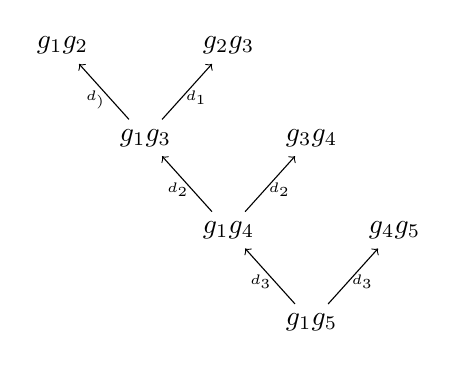
\begin{tikzpicture} [->, baseline=(current bounding box.center)]
    \node {$\subrulep{g_1}{g_5}$} [grow' = up, align=center, anchor=north,
                     sibling distance = 6em, level distance = 4em]
    child {node {$\subrulep{g_1}{g_4}$} 
      child {node {$\subrulep{g_1}{g_3}$}
        child {node {$\subrulep{g_1}{g_2}$} edge from parent
                           node[below left=-0.4em] {$\scriptscriptstyle d_)$}
              }
        child {node {$\subrulep{g_2}{g_3}$} edge from parent
                          node[below right=-0.4em] {$\scriptscriptstyle d_1$}
              }
          edge from parent node[below left=-0.4em] {$\scriptscriptstyle d_2$}
           }
      child {node {$\subrulep{g_3}{g_4}$} edge from parent
                         node[below right=-0.4em] {$\scriptscriptstyle d_2$}}
          edge from parent node[below left=-0.4em] {$\scriptscriptstyle d_3$}
            }
    child {node {$\subrulep{g_4}{g_5}$} edge from parent 
                       node[below right=-0.4em] {$\scriptscriptstyle d_3$}
          };
    \end{tikzpicture}
    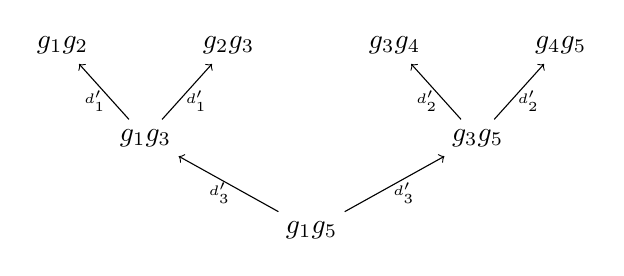
\begin{tikzpicture} [->, baseline=(current bounding box.center)]
    \node {$\subrulep{g_1}{g_5}$} [grow' = up, align=center, anchor=north,
                     sibling distance = 12em, level distance = 4em]
    child {node {$\subrulep{g_1}{g_3}$} [sibling distance=6em]
      child {node {$\subrulep{g_1}{g_2}$}
       edge from parent node[below left=-0.4em] {$\scriptscriptstyle d_1'$}
            }
      child {node {$\subrulep{g_2}{g_3}$}
       edge from parent node[below right=-0.4em] {$\scriptscriptstyle d_1'$}
            }
       edge from parent node[below left=-0.4em] {$\scriptscriptstyle d_3'$}
          }
    child {node {$\subrulep{g_3}{g_5}$} [sibling distance=6em]
      child {node {$\subrulep{g_3}{g_4}$}
       edge from parent node[below left=-0.4em] {$\scriptscriptstyle d_2'$}
            }
      child {node {$\subrulep{g_4}{g_5}$}
       edge from parent node[below right=-0.4em] {$\scriptscriptstyle d_2'$}
            }
       edge from parent node[below right=-0.4em] {$\scriptscriptstyle d_3'$}
          };
    \end{tikzpicture}
    \caption{Vertex-edge representations for (\ref{def:ruleproofnot}-3) and
                   (\ref{def:ruleproofnot}-4)}\label{fig:verep}
     \end{figure}
 \end{metalabpara}


 \begin{metalabpara}{mydefinition}{}
    {Swapped inference rules in vertex-edge format}\envlabel{def:irulegraphswap}
    Given an inference rule $r$, the representation of
$\rswap{r}{\alpha_i}$ is, in principle, straightforward, as
illustrated in (\ref{def:irulegraphswap}-1).  All that is necessary is
to swap the identities of the vertex labelled $\alpha_i$ with that of
the conclusion $\beta$, and negate each.  The edges remain fixed; thus, this representation is called \emph{fixed-edge positioning}.
   \def\transto#1{\hspace*{#1} &\rightsquigarrow \hspace*{#1}}
   \def\sepval{0.5cm}
    \begin{align*}
    \tag{\ref{def:irulegraphswap}-1}
    \begin{tikzpicture} [->, baseline=(current bounding box.center) ]
    \node {$\beta$} [grow' = up, align=center,
                     sibling distance = 2em, level distance = 3em]
    child {node {$\alpha_1$}}
    child {node {$\alpha_2$} edge from parent node [right] {$\ldots$}}
    child {node {$\ldots$} \efpn}
    child {node {$\alpha_{i-1}$}}
    child {node {$\alpha_i$}}
    child {node {$\alpha_{i+1}$} edge from parent node [right] {$\ldots$}}
    child {node {$\ldots$} \efpn}
    child {node {$\alpha_{k-1}$}}
    child {node {$\alpha_k$}};
    \end{tikzpicture}
     \transto{\sepval}
    \begin{tikzpicture} [->, baseline=(current bounding box.center) ]
    \node {$\mlnot\alpha_i$} [grow' = up, align=center,
                     sibling distance = 2em, level distance = 3em]
    child {node {$\alpha_1$}}
    child {node {$\alpha_2$} edge from parent node [right] {$\ldots$}}
    child {node {$\ldots$} \efpn}
    child {node {$\alpha_{i-1}$}}
    child {node {$\mlnot\beta$}  edge from parent []}
    child {node {$\alpha_{i+1}$} edge from parent node [right] {$\ldots$}}
    child {node {$\ldots$} \efpn}
    child {node {$\alpha_{k-1}$}}
    child {node {$\alpha_k$}};
    \end{tikzpicture}
    \end{align*}
   While this works fine for an isolated inference rule, it leads to
problems when such rules are interconnected to form proofs because
vertices must be moved around, creating a representational maze.  It
is more suitable to keep the position of the vertices fixed, and move
the edges as necessary.  This \emph{fixed-vertex positioning} is shown
in (\ref{def:irulegraphswap}-2).
   \def\sepval{0.5cm}
    \begin{align*}
    \begin{tikzpicture} [->, baseline=(current bounding box.center) ]
    \node {$\beta$} [grow' = up, align=center,
                     sibling distance = 2em, level distance = 3em]
    child {node {$\alpha_1$}}
    child {node {$\alpha_2$} edge from parent node [right] {$\ldots$}}
    child {node {$\ldots$} \efpn}
    child {node {$\alpha_{i-1}$}}
    child {node {$\alpha_i$}}
    child {node {$\alpha_{i+1}$} edge from parent node [right] {$\ldots$}}
    child {node {$\ldots$} \efpn}
    child {node {$\alpha_{k-1}$}}
    child {node {$\alpha_k$}};
    \end{tikzpicture}
     \transto{\sepval}
    \tag{\ref{def:irulegraphswap}-2}
%    \def\equivto#1{\hspace*{#1} &\equiv \hspace*{#1}}
%     \equivto{\sepval}\hspace*{0.5em}
    \begin{tikzpicture} [->, baseline=(current bounding box.center),
                         inner sep=0em ]
    \node {$\mlnot\beta$} [grow' = up, align=center,
                     sibling distance = 2em, level distance = 3em]
    child {node (a1)   {$\alpha_1$} \efpn}
    child {node (a2)   {$\alpha_2$} \efpn}
    child {node (ld1)  {$\ldots$} \efpn}
    child {node (aim1) {$\alpha_{i-1}$} \efpn}
    child {node (ai)   {$\mlnot\alpha_i$} edge from parent [<-] }
    child {node (aip1) {$\alpha_{i+1}$} \efpn}
    child {node (ld2)  {$\ldots$} \efpn}
    child {node (akm1) {$\alpha_{k-1}$} \efpn}
    child {node (ak)   {$\alpha_k$} \efpn};
    \draw (ai.250) to[myncbar, arm=0.6,angle=270] (a1.south);
    \draw (ai.235) to[myncbar, arm=0.4,angle=270] (a2.south);
    \draw (ai.220) to[myncbar, arm=0.2,angle=270] (aim1.south);
    \draw (ai.320) to[ myncbar, arm=0.2,angle=270] (aip1.south);
    \draw (ai.305) to[myncbar, arm=0.4,angle=270] (akm1.south);
    \draw (ai.290) to[myncbar, arm=0.6,angle=270] (ak.south);
    \node [below=6pt of ld1] {$\ldots$};
    \node [below=6pt of ld2] {$\ldots$};
    \end{tikzpicture}
    \end{align*}
   Although the vertices $\alpha_i$ and $\beta$ have been negated, all
retain their original positions.  On the other hand, the edges must be
redrawn.  In addition to reversing the original arrow from $\beta$ to
$\alpha_i$, each edge from $\beta$ to $\alpha_j$ for $j\neq i$ is
replaced by an edge from $\alpha_i$ to $\alpha_j$.
 \end{metalabpara}
    

 \begin{metalabpara}{mydefinition}{}
    {Swapping of rule instances}\envlabel{def:swapinst}
     The notion of swapping introduced in \envref{def:ruleswap}
extends naturally to rule instances.  Specifically, if $d$ is an
instance of rule $r$ obtained via substitution $s$ (see
\envref{disc:semwff} and \envref{def:ruleproofnot}), then for
 $\alpha_i \in \antecedentsof{r}$, $\rswap{d}{\substgr{\alpha_i}{s}}$
is the rule instance obtained by applying $s$ to all entries of
$\rswap{r}{\alpha_i}$.
 \end{metalabpara}


 \begin{metalabpara}{notation}{}
    {Proof trees in multiple-use contexts}\envlabel{not:multuse}
     In order to describe the process of proof contrapositioning (see
\envref{def:proofflip}), it is necessary to have a means of
identifying the vertices of the proof tree unambiguously.  For the
case of single-use proofs, this is an easy task, since the WFF
associated with that vertex identifies it uniquely.  However, if the
proof is not single use, there may several vertices labelled with the
same WFF.  In that case, the solution is to identify a non-root vertex
as a pair $\abr{\alpha,d}$ in which $\alpha$ is the WFF and $d$ is the
rule for which $\alpha \in \antecedentsof{d}$.  The root vertex is
identified specially as $\abr{\beta,\textsf{root}}$.  As a concrete
example, consider the proof tree of (\ref{def:single}-1), which is
shown in Fig.\ \ref{fig:multvertex}.
    \begin{figure}[htb]
    \begin{center}
    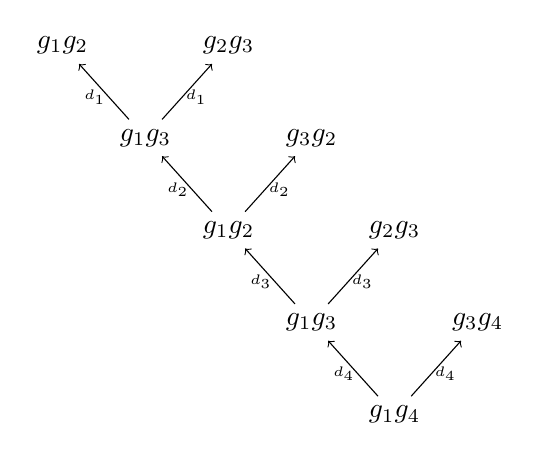
\begin{tikzpicture} [->, baseline=(current bounding box.center)]
    \node {$\subrulep{g_1}{g_4}$} [grow' = up, align=center, anchor=north,
                     sibling distance = 6em, level distance = 4em]
    child {node {$\subrulep{g_1}{g_3}$} 
      child {node {$\subrulep{g_1}{g_2}$}
        child {node {$\subrulep{g_1}{g_3}$}
           child {node {$\subrulep{g_1}{g_2}$} edge from parent
                  node[below left=-0.4em] {$\scriptscriptstyle d_1$}
                 }
           child {node {$\subrulep{g_2}{g_3}$} edge from parent
                  node[below right=-0.4em] {$\scriptscriptstyle d_1$}
                 }
          edge from parent node[below left=-0.4em] {$\scriptscriptstyle d_2$}
              }
        child {node {$\subrulep{g_3}{g_2}$} edge from parent
                          node[below right=-0.4em] {$\scriptscriptstyle d_2$}
              }
          edge from parent node[below left=-0.4em] {$\scriptscriptstyle d_3$}
           }
      child {node {$\subrulep{g_2}{g_3}$} edge from parent
                         node[below right=-0.4em] {$\scriptscriptstyle d_3$}}
          edge from parent node[below left=-0.4em] {$\scriptscriptstyle d_4$}
            }
    child {node {$\subrulep{g_3}{g_4}$} edge from parent 
                       node[below right=-0.4em] {$\scriptscriptstyle d_4$}
          };
    \end{tikzpicture}
    \caption{Vertex-edge representation for
                             (\ref{def:single}-1)}\label{fig:multvertex}
    \end{center}
     \end{figure}
     There are two vertices labelled $\subrulep{g_1}{g_2}$; one is a
leaf, an antecedent of rule $d_1$, while the second is an interior
vertex, an antecedent of rule $d_3$.  These are represented as
$\grpr{\subrulep{g_1}{g_2}}{d_1}$ and $\grpr{\subrulep{g_1}{g_2}}{d_3}$,
respectively.  Note that the root vertex is denoted
$\grpr{\subrulep{g_1}{g_4}}{\textsf{root}}$.
     \par
     Given a proof tree $\tau$, notation such as
 $\grpr{\alpha}{d} \in \antecedentsof{\tau}$ will be used with the
obvious meaning --- that $\alpha \in \antecedentsof{\tau}$.
     \par
    It should be observed that this convention assumes that a single
rule instance does not have multiple instances of the same antecedent.
In most situations, this is a reasonable assumption.  To work with
multiple instances of the same antecedent, it is necessary to employ
trees which have ordered vertices, and to tag the instances with an
index based upon that order.  The details are straightforward, but
will not be used in this work, because they would render the
presentation much more complex.
 \end{metalabpara}


 \begin{metalabpara}{mydefinition}{}
    {Proof contrapositioning}\envlabel{def:proofflip}
  Figs.\ \ref{fig:tocontrap}, \ref{fig:contrapi}, and
\ref{fig:contrapii} illustrate the strategy of \emph{proof
contrapositioning}, in which rule swapping is applied to an entire
proof tree.  Figure \ref{fig:tocontrap} shows a \emph{source tree},
call it $\tau$, in vertex-edge format.
     \begin{figure}[htb]
      \def\markneg#1{#1}
     \def\hsepc{\hspace*{1em}}
%     \def\hsepc{\relax}
    \begin{tikzpicture} [->, baseline=(current bounding box.center) ]
    \node {$\beta$} [grow' = up, align=center, anchor=north,
                     sibling distance = 4em, level distance = 7em]
    child {node {$\treeupps{T_{k1}}$} \efpas
            \edgelabelds{left}{0.3}{near end}{k}
          }
    child {node {$\treeupps{T_{k2}}$} \efpas
            \edgelabelds{right}{0.1}{near end}{k} \noderldots{1.75}
          }
    child {node [below=2em] {$\ldots$} \efpn
          }
    child {node {$\treeupps{T_{k({j_k}\shortminus1)}}$} \efpas
            \edgelabelds{right}{0.1}{near end}{k}
          }
    child {node {$\alpha_{k{j_k}}$} \efpas
     child {node {$\treeupps{T_{(k\shortminus1)1}}$} \efpas
            \edgelabelds{left}{0.1}{near end}{k\shortminus1}
           }
     child {node {$\treeupps{T_{(k\shortminus1)2}}$} \efpas \noderldots{1.75}
            \edgelabelds{right}{0.1}{near end}{k\shortminus1}
           }
     child {node [below=2em] {$\ldots$} \efpn}
     child {node [xshift=-1em]
            {$\treeuppsb{T_{(k\shortminus1)({j_{k\shortminus1}\shortminus1)}}}$} \efpas
            \edgelabelds{right}{0.1}{near end}{k\shortminus1}
           }
     child {node (akm1jkm1) {$\alpha_{(k\shortminus1)(j_{k\shortminus1})}$} \efpas
            \edgelabelds{left}{-0.1}{midway}{k\shortminus1}
           }
     child {node [xshift=1em]
                    {$\treeuppsb{T_{(k\shortminus1)({j_{k\shortminus1}}+1)}}$} \efpas
                                                      \noderldots{1.75}
             node [left=0.1, near end] {$\scriptstyle d_{k\shortminus1}$}
           }
     child {node [below=2em] {$\ldots$} \efpn}
     child {node [xshift=-1em]
            {$\treeuppsb{T_{(k\shortminus1)({m_{k\shortminus1}}\shortminus1)}}$} \efpas
            \edgelabelds{left}{0.1}{near end}{k\shortminus1}
           }
     child {node {$\treeuppsb{T_{(k\shortminus1)(m_{k\shortminus1})}}$} \efpas
            \edgelabelds{right}{0.3}{near end}{k\shortminus1}
           }
            node [left=0.0, midway] {$\scriptstyle d_k$}
            \edgelabelds{left}{0.0}{midway}{k}
          }
    child {node {$\treeupps{T_{k({j_k}+1)}}$} \efpas \noderldots{1.75}
            \edgelabelds{left}{0.1}{near end}{k}
           }
    child {node [below=2em] {$\ldots$} \efpn}
    child {node {$\treeupps{T_{k({m_k}\shortminus1)}}$} \efpas
            \edgelabelds{left}{0.3}{near end}{k}
          }
    child {node {$\treeupps{T_{k{m_k}}}$} \efpas
            \edgelabelds{right}{0.3}{near end}{k}
          };
    \node (vdots1) [ above=1em of akm1jkm1] {$\vdots$};
    \draw (akm1jkm1) -- (vdots1)
            \edgelabelds{right}{-0.1}{midway}{k\shortminus2} ;
    \node (aip1jip1) [above=1em of vdots1]  {$\alpha_{(i+1)(j_{i+1})}$}
                    [grow' = up, align=center, anchor=north,
                     sibling distance = 4em, level distance = 7em]
    child {node {$\treeupps{T_{i1}}$} \efpas
            \edgelabelds{left}{0.3}{near end}{i}
          }
    child {node {$\treeupps{T_{i2}}$} \efpas
            \edgelabelds{right}{0.1}{near end}{i} \noderldots{1.75}
          }
    child {node [below=2em] {$\ldots$} \efpn}
    child {node {$\treeupps{T_{i({j_i}\shortminus1)}}$} \efpas
            \edgelabelds{right}{0.1}{near end}{i}
          }
    child {node (aiji) {$\alpha_{i{j_i}}$} \efpas
            \edgelabelds{left}{-0.1}{midway}{i}
          }
    child {node {$\treeupps{T_{i({j_i}+1)}}$} \efpas \noderldots{1.75}
            \edgelabelds{left}{0.1}{near end}{i}
          }
    child {node [below=2em] {$\ldots$} \efpn}
    child {node {$\treeupps{T_{i({m_i}\shortminus1)}}$} \efpas
            \edgelabelds{left}{0.1}{near end}{i}
          }
    child {node {$\treeupps{T_{i{m_i}}}$} \efpas
            \edgelabelds{right}{0.1}{near end}{i}
          };
    \draw (vdots1) -- (aip1jip1)
            \edgelabelds{right}{-0.1}{midway}{i+1} ;
    \node (vdots2) [ above=1em of aiji] {$\vdots$};
    \draw (aiji) -- (vdots2)
            \edgelabelds{right}{-0.1}{midway}{i\shortminus1} ;
    \node (a3j3) [above=1em of vdots2] {$\alpha_{3{j_3}}$}
                    [grow' = up, align=center, anchor=north,
                     sibling distance = 4em, level distance = 7em]
    child {node {$\treeupps{T_{21}}$} \efpas
            \edgelabelds{left}{0.3}{near end}{2}
          }
    child {node {$\treeupps{T_{22}}$} \efpas
            \edgelabelds{right}{0.3}{near end}{2} \noderldots{1.75}
          }
    child {node [below=2em] {$\ldots$} \efpn}
    child {node {$\treeupps{T_{2({j_2}\shortminus1)}}$} \efpas
            \edgelabelds{right}{0.1}{near end}{2}
          }
    child {node (a2ji) {$\alpha_{2{j_2}}$} \efpas
     child {node {$\treeupps{T_{11}}$} \efpas
            \edgelabelds{left}{0.1}{near end}{1}
           }
     child {node {$\treeupps{T_{12}}$} \efpas
            \edgelabelds{right}{0.3}{near end}{1} \noderldots{1.75}
           }
     child {node [below=2em] {$\ldots$} \efpn}
     child {node {$\treeupps{T_{1({j_1}\shortminus1)}}$} \efpas
            \edgelabelds{right}{0.1}{near end}{1}
           }
     child {node (a1j1) {$\alpha_{1{j_1}}$} \efpas
            \edgelabelds{left}{-0.1}{midway}{1}
           }
     child {node {$\treeupps{T_{1({j_1}+1)}}$} \efpas
            \edgelabelds{left}{0.1}{near end}{1} \noderldots{1.75}
           } 
     child {node [below=2em] {$\ldots$} \efpn}
     child {node {$\treeupps{T_{1({m_1}\shortminus1)}}$} \efpas
            \edgelabelds{left}{0.1}{near end}{1}
           }
     child {node {$\treeupps{T_{1m_1}}$} \efpas
            \edgelabelds{right}{0.3}{near end}{1}
           }
            \edgelabelds{left}{-0.1}{midway}{2}
          }
    child {node {$\treeupps{T_{2({j_2}+1)}}$} \efpas
            \edgelabelds{left}{0.1}{near end}{2} \noderldots{1.75}
          }
    child {node [below=2em] {$\ldots$} \efpn}
    child {node {$\treeupps{T_{2({m_2}\shortminus1)}}$} \efpas
            \edgelabelds{left}{0.1}{near end}{2}
          }
    child {node {$\treeupps{T_{2{m_2}}}$} \efpas
            \edgelabelds{right}{0.3}{near end}{2}
          };
    \draw (vdots2) to (a3j3);
    \end{tikzpicture}
    \caption{The source proof to undergo contrapositioning}\label{fig:tocontrap}
    \end{figure}
     It is an arbitrary proof tree using the rules $\proofsys{A}$; no
special properties are assumed.  Each entry of the form
{\footnotesize$\treeup{T_{ij}}$} represents a subtree of the entire
proof tree which remains unchanged during the transformation.
    The most important vertex in the tree is
$\grpr{\alpha_{1{j_1}}}{d_1}$, called the \emph{(designated) swap
leaf} of $\tau$.  It is the antecedent which will be swapped with the
consequent $\beta$ to obtain a proof of $\mlnot\alpha_{1{j_1}}$ from
 $(\antecedentsof{\tau} \setminus \setbr{\alpha_{1{j_1}}})
                               \union \setbr{\mlnot\beta}$.
   The \emph{swap path} is
 \nlrightt
    $\abr{\grpr{\alpha_{1{j_1}}}{d_1},\grpr{\alpha_{2{j_2}}}{d_2},
          \ldots,\grpr{\alpha_{i{j_i}}}{d_i},\ldots,
          \grpr{\alpha_{(k-1){j_{k-1}}}}{d_{i-1}},
          \grpr{\alpha_{k{j_k}}}{d_k},\grpr{\beta}{\rootv}}$,
  \linebreak
  the (unique) path from the swap leaf to the root.  The members of
this sequence are precisely the vertices whose assertions will be
negated in the contrapositioned proof.  In Fig.\ \ref{fig:tocontrap},
this path goes right down the middle of the diagram.
%   The \emph{swap-rule sequence} $\abr{d_{1},d_{2},\ldots,d_{k}}$
%identifies the proof rules associated with the vertices of the swap
%path.
     For  $i \in \ccinterval{1}{k-1}$, 
         $\consequentof{d_{i}} = \alpha_{(i+1){j_{i+1}}}
                             \in \antecedentsof{d_{i+1}}$,
 with
 $\consequentof{d_{k}} = \beta$.
    \par
  In the result, called the \emph{contrapositioned tree}, each rule
instance $d_{i}$ in the swap-rule sequence is replaced by
 $\rswap{d_{i}}{\alpha_{i{j_i}}}$.  This tree is illustrated in
Fig.\ \ref{fig:contrapi}, using fixed-vertex positioning as described
in \envref{def:irulegraphswap}.  For compactness of notation, this
replacement rule is labelled $d_{i}'$ in Fig.\ \ref{fig:contrapi}.
     \begin{figure}[htb]
      \def\markneg#1{#1}
     \def\hsepc{\hspace*{1em}}
   \begin{tikzpicture} [->, baseline=(current bounding box.center) ]
    \node (beta) {$\mlnot\beta$} [grow' = up, align=center, anchor=north,
                     sibling distance = 4em, level distance = 7em]
    child {node (tk1) {$\treeupps{T_{k1}}$} \efpn}
    child {node (tk2) {$\treeupps{T_{k2}}$} \efpn}
    child {\nodebldots{0.5} \efpn}
    child {node (tkjkm1) {$\treeupps{T_{k({j_k}\shortminus1)}}$} \efpn}
    child {node (akjk) {$\mlnot\alpha_{k{j_k}}$} edge from parent [<-]
     child {node (tkm11) {$\treeupps{T_{(k\shortminus1)1}}$} \efpn}
     child {node (tkm12) {$\treeupps{T_{(k\shortminus1)2}}$} \efpn}
     child {\nodebldots{0.5} \efpn}
     child {node (tkm1jkm1m1) [xshift=-1em]
            {$\treeuppsb{T_{(k\shortminus1)({j_{k\shortminus1}\shortminus1)}}}$} \efpn}
     child {node (akm1jkm1) {$\mlnot\alpha_{(k\shortminus1)(j_{k\shortminus1})}$}
                                     edge from parent [<-]
           \edgelabeldsp{left}{-0.1}{very near start}{k\shortminus1}
           }
     child {node (tkm1jkm1p1) [xshift=1em]
             {$\treeuppsb{T_{(k\shortminus1)({j_{k\shortminus1}}+1)}}$} \efpn}
     child {\nodebldots{0.5} \efpn}
     child {node (tkm1mkm1m1) [xshift=-1em]
            {$\treeuppsb{T_{(k\shortminus1)({m_{k\shortminus1}}\shortminus1)}}$} \efpn}
     child {node (tkm1mkm1) {$\treeuppsb{T_{(k\shortminus1)(m_{k\shortminus1})}}$}
            \efpn
           }
           \edgelabeldsp{left}{-0.1}{very near start}{k}
          }
    child {node (tkjkp1) {$\treeupps{T_{k({j_k}+1)}}$} \efpn}
    child {\nodebldots{0.5} \efpn}
    child {node (tkmkm1) {$\treeupps{T_{k({m_k}\shortminus1)}}$} \efpn}
    child {node (tkmk) {$\treeupps{T_{k{m_k}}}$} \efpn};
%%% T1x
    \draw (akm1jkm1.250) to[myncbar, arm=1.45,angle=270]
            node[left] {\edgelabelnames{d_{k\shortminus1}'}} (tkm11.south);
    \draw (akm1jkm1.235) to[myncbar, arm=1.35,angle=270]
            node[left] {\edgelabelnames{d_{k\shortminus1}'}} (tkm12.south);
    \draw (akm1jkm1.220) to[myncbar, arm=1.25,angle=270]
            node[left] {\edgelabelnames{d_{k\shortminus1}'}} (tkm1jkm1m1.south);
    \draw (akm1jkm1.320) to[myncbar, arm=1.25,angle=270]
            node[right] {\edgelabelnames{d_{k\shortminus1}'}} (tkm1jkm1p1.south);
    \draw (akm1jkm1.305) to[myncbar, arm=1.35,angle=270]
            node[right] {\edgelabelnames{d_{k\shortminus1}'}} (tkm1mkm1m1.south);
    \draw (akm1jkm1.290) to[myncbar, arm=1.45,angle=270]
            node[right] {\edgelabelnames{d_{k\shortminus1}'}} (tkm1mkm1.south);
%%% T2x
    \draw (akjk.250) to[myncbar, arm=1.45,angle=270]
            node[left] {\edgelabelnames{d_{k}'}} (tk1.south);
    \draw (akjk.235) to[myncbar, arm=1.35,angle=270]
            node[left] {\edgelabelnames{d_{k}'}} (tk2.south);
    \draw (akjk.220) to[myncbar, arm=1.25,angle=270]
            node[left] {\edgelabelnames{d_{k}'}} (tkjkm1.south);
    \draw (akjk.320) to[myncbar, arm=1.25,angle=270]
            node[right] {\edgelabelnames{d_{k}'}} (tkjkp1.south);
    \draw (akjk.305) to[myncbar, arm=1.35,angle=270]
            node[right] {\edgelabelnames{d_{k}'}} (tkmkm1.south);
    \draw (akjk.290) to[myncbar, arm=1.45,angle=270]
            node[right] {\edgelabelnames{d_{k}'}} (tkmk.south);
    \node (vdots1) [ above=1em of akm1jkm1] {$\vdots$};
    \draw [<-] (akm1jkm1) -- (vdots1)
           \edgelabeldsp{left}{-0.1}{midway}{k\shortminus2};
    \node (aip1jip1) [above=1em of vdots1]  {$\mlnot\alpha_{(i+1)(j_{i+1})}$}
                    [grow' = up, align=center, anchor=north,
                     sibling distance = 4em, level distance = 7em]
    child {node (ti1) {$\treeupps{T_{i1}}$}
                    edge from parent [child anchor=south, draw=none]}
    child {node (ti2) {$\treeupps{T_{i2}}$}
                    edge from parent [child anchor=south, draw=none]}
    child {\nodebldots{0.5} \efpn}
    child {node (tijim1) {$\treeupps{T_{i({j_i}\shortminus1)}}$}
                    edge from parent [child anchor=south, draw=none]}
    child {node (aiji) {$\mlnot\alpha_{i{j_i}}$} edge from parent [<-]
           \edgelabeldsp{left}{-0.1}{very near start}{i}          }
    child {node (tijip1) {$\treeupps{T_{i({j_i}+1)}}$}
                    edge from parent [child anchor=south, draw=none]}
    child {\nodebldots{0.5} \efpn}
    child {node (timim1) {$\treeupps{T_{i({m_i}\shortminus1)}}$}
                    edge from parent [child anchor=south, draw=none]}
    child {node (timi) {$\treeupps{T_{i{m_i}}}$}
                    edge from parent [child anchor=south, draw=none]};
%%% Tix
    \draw (aiji.250) to[myncbar, arm=1.45,angle=270]
            node[left] {\edgelabelnames{d_{i}'}} (ti1.south);
    \draw (aiji.235) to[myncbar, arm=1.35,angle=270]
            node[left] {\edgelabelnames{d_{i}'}} (ti2.south);
    \draw (aiji.220) to[myncbar, arm=1.25,angle=270]
            node[left] {\edgelabelnames{d_{i}'}} (tijim1.south);
    \draw (aiji.320) to[myncbar, arm=1.25,angle=270]
            node[right] {\edgelabelnames{d_{i}'}} (tijip1.south);
    \draw (aiji.305) to[myncbar, arm=1.35,angle=270]
            node[right] {\edgelabelnames{d_{i}'}} (timim1.south);
    \draw (aiji.290) to[myncbar, arm=1.45,angle=270]
            node[right] {\edgelabelnames{d_{i}'}} (timi.south);
    \draw [<-] (vdots1) -- (aip1jip1)
           \edgelabeldsp{left}{-0.1}{midway}{i+1};
    \node (vdots2) [ above=1em of aiji] {$\vdots$};
    \draw [<-] (aiji) -- (vdots2)
           \edgelabeldsp{left}{-0.1}{midway}{i\shortminus1};
    \node (a3j3) [above=1em of vdots2] {$\mlnot\alpha_{3{j_3}}$}
                    [grow' = up, align=center, anchor=north,
                     sibling distance = 4em, level distance = 7em]
    child {node (t21) {$\treeupps{T_{21}}$}
                edge from parent [child anchor=south,draw=none]}
    child {node (t22) {$\treeupps{T_{22}}$}
                edge from parent [child anchor=south,draw=none]}
    child {\nodebldots{0.5} \efpn}
    child {node (t2j2m1) {$\treeupps{T_{2({j_2}\shortminus1)}}$}
                edge from parent [child anchor=south,draw=none]}
    child {node (a2j2) {$\mlnot\alpha_{2{j_2}}$} edge from parent [<-] 
     child {node (t11) {$\treeupps{T_{11}}$}
                edge from parent [child anchor=south,draw=none]}
     child {node (t12) {$\treeupps{T_{12}}$}
                edge from parent [child anchor=south,draw=none]}
     child {\nodebldots{0.5} \efpn}
     child {node (t1jm1) {$\treeupps{T_{1({j_1}\shortminus1)}}$}
                edge from parent [child anchor=south,draw=none]}
     child {node (a1j1) {$\mlnot\alpha_{1{j_1}}$} edge from parent [<-]
           \edgelabeldsp{left}{-0.1}{very near start}{1}
           }
     child {node (t1j1p1) {$\treeupps{T_{1({j_1}+1)}}$}
                edge from parent [child anchor=south,draw=none]}
     child {\nodebldots{0.5} \efpn}
     child {node (t1m1m1) {$\treeupps{T_{1({m_1}\shortminus1)}}$}
                edge from parent [child anchor=south,draw=none]}
     child {node (t1m1) {$\treeupps{T_{1m_1}}$}
                edge from parent [child anchor=south,draw=none]}
           \edgelabeldsp{left}{-0.1}{very near start}{2}
          }
    child {node (t2j2p1) {$\treeupps{T_{2({j_2}+1)}}$}
                edge from parent [child anchor=south,draw=none]}
    child {\nodebldots{0.5} \efpn}
    child {node (t2m2m1) {$\treeupps{T_{2({m_2}\shortminus1)}}$}
                edge from parent [child anchor=south,draw=none]}
    child {node (t2m2) {$\treeupps{T_{2{m_2}}}$}
               edge from parent [child anchor=south,draw=none]};
    \draw [<-] (vdots2) -- (a3j3)
           \edgelabeldsp{left}{-0.1}{midway}{3};
%%% T1x
    \draw (a1j1.250) to[myncbar, arm=1.45,angle=270]
            node[left] {\edgelabelnames{d_{1}'}} (t11.south);
    \draw (a1j1.235) to[myncbar, arm=1.35,angle=270]
            node[left] {\edgelabelnames{d_{1}'}} (t12.south);
    \draw (a1j1.220) to[myncbar, arm=1.25,angle=270]
            node[left] {\edgelabelnames{d_{1}'}} (t1jm1.south);
    \draw (a1j1.290) to[myncbar, arm=1.45,angle=270]
            node[right] {\edgelabelnames{d_{1}'}} (t1m1.south);
    \draw (a1j1.305) to[myncbar, arm=1.35,angle=270]
            node[right] {\edgelabelnames{d_{1}'}} (t1m1m1.south);
    \draw (a1j1.320) to[myncbar, arm=1.25,angle=270]
            node[right] {\edgelabelnames{d_{1}'}} (t1j1p1.south);
%%% T2x
    \draw (a2j2.250) to[myncbar, arm=1.45,angle=270]
            node[left] {\edgelabelnames{d_{2}'}} (t21.south);
    \draw (a2j2.235) to[myncbar, arm=1.35,angle=270]
            node[left] {\edgelabelnames{d_{2}'}} (t22.south);
    \draw (a2j2.220) to[myncbar, arm=1.25,angle=270]
            node[left] {\edgelabelnames{d_{2}'}} (t2j2m1.south);
    \draw (a2j2.320) to[myncbar, arm=1.25,angle=270]
            node[right] {\edgelabelnames{d_{2}'}} (t2j2p1.south);
    \draw (a2j2.305) to[myncbar, arm=1.35,angle=270]
            node[right] {\edgelabelnames{d_{2}'}} (t2m2m1.south);
    \draw (a2j2.290) to[myncbar, arm=1.45,angle=270]
            node[right] {\edgelabelnames{d_{2}'}} (t2m2.south);
    \end{tikzpicture}
     \caption{The contrapositioned proof in fixed-position format}\label{fig:contrapi}
     \end{figure}
    Notice that the changes described in \envref{def:irulegraphswap}
are followed.  In particular, in the transition from $d_i$ to $d_i'$,
the antecedent $\alpha_{i{j_i}}$ and the consequent
$\alpha_{(i+1){j_{i+1}}}$ ($\beta$ for $d_k$) are negated, and the
arrow connecting them is reversed.  Furthermore, the source of all
arrows of $d_i$ is changed to $\mlnot\alpha_{i{j_i}}$ in $d_i'$.
     \par
     In Fig,\ \ref{fig:contrapii}, this same contrapositioned tree is
shown in fixed-edge format.  
     \begin{figure}[htb]
      \def\markneg#1{#1}
     \def\hsepc{\hspace*{1em}}
    \begin{tikzpicture} [->, baseline=(current bounding box.center) ]
    \node {$\mlnot\alpha_{1{j_1}}$} [grow' = up, align=center, anchor=north,
                     sibling distance = 4em, level distance = 7em]
    child {node {$\treeupps{T_{11}}$} \efpas
            \edgelabeldsp{left}{0.3}{near end}{1}
          }
    child {node {$\treeupps{T_{12}}$} \efpas
            \edgelabeldsp{right}{0.1}{near end}{1}
                                     node [right=1.75em] {$\ldots$}
          }
    child {node [below=2em] {$\ldots$} \efpn}
    child {node {$\treeupps{T_{1({j_1}\shortminus1)}}$}
                                     \efpas
            \edgelabeldsp{right}{0.1}{near end}{1}
          }
    child {node {$\mlnot\alpha_{2{j_2}}$} \efpas
     child {node {$\treeupps{T_{21}}$}
                                     \efpas
            \edgelabeldsp{left}{0.3}{near end}{2}
           }
     child {node {$\treeupps{T_{22}}$}
                                      \efpas
            \edgelabeldsp{right}{0.1}{near end}{2}
                                      node [right=1.75em] {$\ldots$}
           }
     child {node [below=2em] {$\ldots$} \efpn}
     child {node {$\treeupps{T_{2(j_2\shortminus1)}}$}
                                     \efpas
            \edgelabeldsp{right}{0.1}{near end}{2}
           }
     child {node (akm1jkm1) {$\mlnot\alpha_{3j_3}$} \efpas
            \edgelabeldsp{left}{-0.1}{midway}{2}
           }
     child {node {$\treeupps{T_{2({j_2}+1)}}$} \efpas
                                     node [right=1.75em] {$\ldots$}
            \edgelabeldsp{left}{0.3}{near end}{2}
           } 
     child {node [below=2em] {$\ldots$} \efpn}
     child {node {$\treeupps{T_{2({m_2}\shortminus1)}}$} \efpas
            \edgelabeldsp{left}{0.3}{near end}{2}
           }
     child {node {$\treeupps{T_{2m_2}}$} \efpas
            \edgelabeldsp{right}{0.5}{near end}{2}
           }
            \edgelabeldsp{left}{-0.1}{midway}{1}
          }
    child {node {$\treeupps{T_{1({j_1}+1)}}$} \efpas
            \edgelabeldsp{left}{0.3}{near end}{1}
                                     node [right=1.75em] {$\ldots$}}
    child {node [below=2em] {$\ldots$} \efpn}
    child {node {$\treeupps{T_{1({m_1}\shortminus1)}}$} \efpas
            \edgelabeldsp{left}{0.3}{near end}{1}
                }
    child {node {$\treeupps{T_{1{m_1}}}$} \efpas
            \edgelabeldsp{right}{0.5}{near end}{1}
          };
    \node (vdots1) [ above=1em of akm1jkm1] {$\vdots$};
    \draw (akm1jkm1) -- (vdots1)
            \edgelabeldsp{left}{-0.1}{midway}{3};
    \node (aip1jip1) [above=1em of vdots1]  {$\mlnot\alpha_{i{j_i}}$}
                    [grow' = up, align=center, anchor=north,
                     sibling distance = 4em, level distance = 7em]
    child {node {$\treeupps{T_{i1}}$} \efpas
            \edgelabeldsp{left}{0.5}{near end}{i}
          }
    child {node {$\treeupps{T_{i2}}$} \efpas
            \edgelabeldsp{right}{0.5}{near end}{i}
                                     node [right=1.75em] {$\ldots$}
          }
    child {node [below=2em] {$\ldots$} \efpn}
    child {node [xshift=-1em] {$\treeupps{T_{i({j_i}\shortminus1)}}$} \efpas
            \edgelabeldsp{right}{0.1}{near end}{i}
          }
    child {node (aiji) {$\mlnot\alpha_{(i+1){j_{i+1}}}$} \efpas
            \edgelabeldsp{left}{-0.1}{midway}{i}
          }
    child {node [xshift=1em] {$\treeupps{T_{i({j_i}+1)}}$} \efpas
            \edgelabeldsp{left}{0.1}{near end}{i}
                                     node [right=1.75em] {$\ldots$}
          }
    child {node [below=2em] {$\ldots$} \efpn}
    child {node {$\treeupps{T_{i({m_i}\shortminus1)}}$} \efpas
            \edgelabeldsp{left}{0.5}{near end}{i}
          }
    child {node {$\treeupps{T_{i{m_i}}}$} \efpas
            \edgelabeldsp{right}{0.5}{near end}{i}
          };
    \draw (vdots1) -- (aip1jip1)
            \edgelabeldsp{left}{-0.1}{midway}{i_1};
    \node (vdots2) [ above=1em of aiji] {$\vdots$};
    \draw (aiji) -- (vdots2)
            \edgelabeldsp{left}{-0.1}{midway}{i+1};
    \node (a3j3) [above=1em of vdots2]
                     {$\mlnot\alpha_{(k\shortminus1){j_{(k\shortminus1)}}}$}
                    [grow' = up, align=center, anchor=north,
                     sibling distance = 4em, level distance = 7em]
    child {node {$\treeupps{T_{(k\shortminus1)1}}$} \efpas
            \edgelabeldsp{left}{0.3}{near end}{k\shortminus1}
          }
    child {node {$\treeupps{T_{(k\shortminus1)2}}$} \efpas
            \edgelabeldsp{right}{0.3}{near end}{k\shortminus1}
                                     node [right=1.75em] {$\ldots$}}
    child {node [below=2em] {$\ldots$} \efpn}
    child {node {$\treeuppsb{T_{(k\shortminus1)({j_{k\shortminus1}}\shortminus1)}}$}
                \efpas
            \edgelabeldsp{right}{0.1}{near end}{k\shortminus1}
          }
    child {node (a2i2) {$\mlnot\alpha_{k{j_k}}$} \efpas
     child {node {$\treeupps{T_{k1}}$} \efpas
            \edgelabeldsp{left}{0.3}{near end}{k}
           }
     child {node {$\treeupps{T_{k2}}$} \efpas
            \edgelabeldsp{right}{0.3}{near end}{k}
                                      node [right=1.75em] {$\ldots$}}
     child {node [below=2em] {$\ldots$} \efpn}
     child {node {$\treeupps{T_{k({j_k}\shortminus1)}}$} \efpas
            \edgelabeldsp{right}{0.3}{near end}{k}
           }
     child {node (a1i1) {$\mlnot\beta$} \efpas
            \edgelabeldsp{left}{-0.1}{midway}{k}
           }
     child {node {$\treeupps{T_{k({j_k}+1)}}$}
                                     \efpas
            \edgelabeldsp{left}{0.3}{near end}{k}
                                     node [right=1.75em] {$\ldots$}} 
     child {node [below=2em] {$\ldots$} \efpn}
     child {node {$\treeupps{T_{k({m_k}\shortminus1)}}$} \efpas
            \edgelabeldsp{left}{0.3}{near end}{k}
           }
     child {node {$\treeupps{T_{1m_k}}$} \efpas
            \edgelabeldsp{right}{0.3}{near end}{k}
           }
            \edgelabeldsp{left}{-0.1}{midway}{k\shortminus1}
          }
    child {node {$\treeuppsb{T_{(k\shortminus1)({j_{k\shortminus1}}+1)}}$} \efpas
            \edgelabeldsp{left}{0.1}{near end}{k\shortminus1}
                                     node [right=1.75em] {$\ldots$}}
    child {node [below=2em] {$\ldots$} \efpn}
    child {node [xshift=-1em]
           {$\treeuppsb{T_{(k\shortminus1)({m_{k\shortminus1}}\shortminus1)}}$} \efpas
            \edgelabeldsp{left}{0.3}{near end}{k\shortminus1}
          }
    child {node {$\treeuppsb{T_{(k\shortminus1){m_{k\shortminus1}}}}$} \efpas
            \edgelabeldsp{right}{0.3}{near end}{k\shortminus1}
          };
    \draw (vdots2) -- (a3j3)
            \edgelabeldsp{left}{-0.1}{midway}{k\shortminus2};
    \end{tikzpicture}
     \caption{The contrapositioned proof in hierarchical format}\label{fig:contrapii}
     \end{figure}
Although the result may seem more aesthetically pleasing, note
that there has been substantial rearrangement --- the swapped rules
occur in the flipped tree in the opposite order from that in the
source tree, since the swapping operation exchanges an antecedent of
the rule with the consequent (and then complements both).  Thus, while
fixed-edge positioning may result in a tree which looks more natural,
it is fixed-vertex positioning which illustrates, in a far more
understandable manner, the relationship between the source tree and its
contrapositioned counterpart.
     \par
     The contrapositioning of the tree $\tau$ is denoted
$\contraposn{\tau}{\grpr{\alpha_{1{j_i}}}{d_1}}$.  The swap leaf
determines the entire swap path.
     \par
     For examples of contrapositioning, the reader is encouraged to
look ahead to \envref{ex:neginf1} and \envref{ex:neginf2}.
     The immediate topic is to establish the key completeness result
surrounding contrapositioning.
 \end{metalabpara}


 \begin{metaemphlabpara}{lemma}{Lemma}
    {Contrapositioning preserves proof}\envlabel{lem:contraptree}
 If $\tau$ is a proof tree over $\proofsys{A}$ with
 $\grpr{\alpha}{d} \in \antecedentsof{\tau}$, then
$\contraposn{\tau}{\grpr{\alpha}{d}}$ is a proof of $\mlnot\alpha$
from
  $(\antecedentsof{\tau} \setminus \setbr{\alpha})
     \union \setbr{\mlnot\consequentof{\tau}}$
 in the proof system $\swapcl{\proofsys{A}}$.
 \begin{proof}
     The result follows directly from the construction given in
\envref{def:proofflip}.  It is easy to verify that
$\contraposn{\tau}{\grpr{\alpha}{d}}$ is a proof tree constructed from
the rules of $\swapcl{\proofsys{A}}$, with the required antecedents
and consequent.
 \end{proof}
 \end{metaemphlabpara}
 
 \begin{metaemphlabpara}{theorem}{Theorem}
    {Sat-completeness of
         Armstrong inference systems}\envlabel{thm:armcomplete}
  If $\proofsys{A}$ is sound, complete and single use, then
$\swapcl{\proofsys{A}}$ is sound, sat-complete, and single use
also.
 \begin{proof}
   Consistency of $\swapcl{\proofsys{A}}$ follows from
\envref{prop:genswap}(b).
   To show sat-completeness, assume that $\proofsys{A}$ is complete,
and let $\Phi \subseteq \allarm{\armctxt{C}}$ be satisfiable, and let
 $\psi \in \armctxt{C}$.  There are two cases to consider: 
 $\Phi \sentails \psi$ and $\Phi \sentails \mlnot\psi$.
     \par
    For the first case, $\Phi \sentails \psi$, it suffices to invoke
\envref{prop:infarm}(a), which ensures that
 $\posof{\Phi} \syntailss[\proofsys{A}] \psi$,
 whence $\Phi \syntailss[\proofsys{A}] \psi$ holds \emph{a fortiori}.
     \par
   For the second case, if $\Phi \sentails \mlnot\psi$, then by
\envref{prop:infarm}(b), either
  $\posof{\Phi} \union \setbr{\psi}
                  \syntailss[\proofsys{A}] \false$,
 or else there is a single
 $\mlnot\varphi \in \negof{\Phi}$ with the property that 
   $\posof{\Phi} \union \setbr{\psi} \sentails \varphi$.
    For the first subcase,  $\posof{\Phi} \union \setbr{\psi}
                  \syntailss[\proofsys{A}] \false$,
 let $\tau$ be the proof tree in $\proofsys{A}$
modelled after that of Fig.\ \ref{fig:tocontrap}, with $\alpha_{1{j_1}}=\psi$
and $\beta=\false$.
    For the second subcase,
     $\posof{\Phi} \union \setbr{\psi} \sentails \varphi$ for some
$\mlnot\varphi \in \negof{\Phi}$, let $\tau$ be the proof tree in
$\proofsys{A}$ modelled after that of Fig.\ \ref{fig:tocontrap}, with
 $\alpha_{1{j_1}}=\psi$ and $\beta=\varphi$.
    In either subcase, the completeness of $\proofsys{A}$ guarantees
that such a tree exists.  If $\psi$ is used more than once as an
antecedent, pick any occurrence.  (It will be shown shortly that such
multiple occurrences are impossible.)
    \par
    Now, consider the tree
$\tau'=\contraposn{\tau}{\grpr{\psi}{d_1}}$, with $d_1$ the rule which
has $\psi=\alpha_{1{j_1}}$ as antecedent, as in
Fig.\ \ref{fig:tocontrap}.  In both subcases identified above, the
contrapositioned tree $\tau'$ will have $\mlnot\psi$ as the
conclusion.  In the first,
 $\mlnot\beta=\mlnot\false=\true$, so $\mlnot\beta$ is simply omitted
as an antecedent of $\tau'$.
    In the second, $\mlnot\beta=\mlnot\varphi$, which is
exactly the single negative sentence which must be added as an
antecedent of the entire proof.
    It cannot be the case that there are multiple occurrences of
$\psi$ in the original tree $\tau$.  If there were, the resulting tree
would exhibit a proof of $\mlnot\psi$ from a set of premises which
includes $\psi$.  Since all of the rules are sound, this is
impossible.
    \par
    From this, it follows that $\contraposn{\tau}{\grpr{\psi}{d_1}}$
is a proof of $\psi$ from $\Phi$ in $\swapcl{\proofsys{A}}$, so the
latter is sat-complete.  The single-use property follows from the
argument of the previous paragraph.
  \end{proof}
 \end{metaemphlabpara}

   \parvert
    To obtain a system which is complete even for unsatisfiable
formulas of $\allarm{\armctxt{C}}$, the notion of complement-pair
rules is introduced.    

 \begin{metalabpara}{mydefinition}{}
    {Complement-pair rules}\envlabel{def:compprrules}
     A \emph{complement-pair rule} is one which asserts that a WFF and
its negation cannot both be true.  A generic such rule is illustrated
in (\ref{def:compprrules}-1).
     \[
       \tag{\ref{def:compprrules}-1}
       \begin{prooftree}
         \hypoii{\alpha}
                {\mlnot\alpha}
         \inferi{\false}
       \end{prooftree}
     \]
    The \emph{complement-pair set} of $\armctxt{C}$, denoted
$\compprset{\armctxt{C}}$, includes, for each
 $\alpha \in \armctxt{C}$, a complement-pair rule of the form shown
(\ref{def:compprrules}-1).  In the case that the rules of
$\proofsys{A}$ are represented generically using variables, it is only
necessary to add rules which instantiate to all complement-pair rules.
For the main example $\pbinconstrgrsch{G}$,
$\compprset{\pbinconstrgrsch{G}}$ is given by the two rules shown in
Fig.\ \ref{fig:cprgrsch}.
  \begin{figure}[htb]
  \begin{center}
   \def\isepi{0.5em}
   \begin{align*}
   &\mbox{(C1)}\hspace*{\isepi}
    \begin{prooftreem}
       \hypoii{\subrulep{\granvar{g}_1}{\granvar{g}_2}}
              {\nsubrulep{\granvar{g}_1}{\granvar{g}_2}}
       \inferi{\false}
    \end{prooftreem}
   &&\mbox{(C2)}\hspace*{\isepi}
    \begin{prooftreem}
      \hypoii{\disjrulep{\granvar{g}_1}{\granvar{g}_2}}
              {\ndisjrulep{\granvar{g}_1}{\granvar{g}_2}}
      \inferi{\false}
    \end{prooftreem}
    \end{align*}
  \end{center}
  \caption{Complement-pair rules for $\pbinconstrgrsch{G}$}\label{fig:cprgrsch}
  \end{figure}
     \par
   The \emph{full swap closure} of $\proofsys{A}$, denoted
$\fullswapcl{\proofsys{A}}$, is
 $\swapcl{A} \union \compprset{\armctxt{C}}$.
    Thus,
     $\fullswapcl{\bininfpos{G}} = \swapcl{\bininfpos{G}} \union
                                  \compprset{\pbinconstrgrsch{G}} =
       \nlrightt
          \setbr{\text{(I2)},   \text{(M1)}, \text{(I1)},
            \text{(T1)},  \text{(T2)},  \text{(T3)},
            \text{(U1},
            \text{(I2-sa)},  \text{(I2-sb)},
                 \text{(M1-sa)}, \text{(M1-sb)},
                 \text{(U1-s)},
            \text{(C1)}, \text{(C2)}
                }$.
     \par
   The justification for this terminology is that a complement-pair
rule may be regarded as the swap of an identity rule, as illustrated
in (\ref{def:compprrules}-2).  The middle inference rule is equivalent
to the leftmost, adding only a $\true$ premise, while the rightmost
rule results from the swap of the antecedent $\true$ and the
consequent $\alpha$.

  \def\sepval{0.5cm}
     \[
       \tag{\ref{def:compprrules}-2}
       \begin{prooftree}
         \hypoi{\alpha}
         \inferi{\alpha}
       \end{prooftree}
     \equivto{\sepval}
       \begin{prooftree}
         \hypoii{\alpha}
                 {\true}
         \inferi{\alpha}
       \end{prooftree}
     \transto{\sepval}
       \begin{prooftree}
         \hypoii{\alpha}
                {\mlnot\alpha}
         \inferi{\false}
       \end{prooftree}
     \]
   Thus, if identity rules, such as the leftmost rule of
(\ref{def:compprrules}-2), were added to $\proofsys{A}$, then the
complement-pair rules would be included in the swap closure.
 \end{metalabpara}


 \begin{metaemphlabpara}{lemma}{Lemma}
    {Characterization of unsatisfiability in
          $\allarm{\armctxt{C}}$}\envlabel{lem:compprrules}
     Let $\Phi \subseteq \allarm{\armctxt{C}}$.  If $\Phi$ is
unsatisfiable, then either $\posof{\Phi}$ is unsatisfiable or else
there is a\/ $\mlnot\varphi \in \negof{\Phi}$ with the property that
$\posof{\Phi} \sentails \varphi$.
 \begin{proof}
     If $\posof{\Phi}$ is unsatisfiable, then applying
\envref{prop:entarm}(b) with
  $\beta \equiv \true$ (so $\mlnot\beta \equiv \false$),
 it follows that either $\posof{\Phi} \sentails \false$;
 \ie, $\posof{\Phi}$ is unsatisfiable, or else there is a 
 $\mlnot\varphi \in \negof{\Phi}$
 with the  property that
 $\posof{\Phi} \union \setbr{\mlnot\varphi} \sentails \false$;
 \ie, that $\posof{\Phi} \union \setbr{\mlnot\varphi}$ is
unsatisfiable.  From this, it follows from \envref{lem:genswap}(a$'$)
that $\posof{\Phi} \sentails \varphi$, as required.
 \end{proof}
 \end{metaemphlabpara}


 \begin{metaemphlabpara}{theorem}{Theorem}
    {Completeness of $\fullswapcl{\proofsys{A}}$}\envlabel{thm:fullswapcompl}
     If $\proofsys{A}$ is complete, then the proof system
$\fullswapcl{\proofsys{A}}$ is both sound and complete.
 \begin{proof}
    Assume that $\proofsys{A}$ is complete.  Soundness and
sat-completeness of $\fullswapcl{\proofsys{A}}$ follow from
\envref{thm:armcomplete}.
    Indeed, the rules of $\compprset{\proofsys{A}}$ are clearly sound,
and adding them to $\swapcl{\proofsys{A}}$  has no effect on
sat-completeness.
    \par
   To show that completeness extends to unsatisfiable inferences, let
 $\Phi \subseteq \allarm{\armctxt{C}}$ be unsatisfiable.  If
$\posof{\Phi}$ is unsatisfiable, then this is already provable using
only the rules of $\proofsys{A}$, since it is assumed to be complete.
Trivially, a proof that $\posof{\Phi}$ is unsatisfiable is also a
proof that all of $\Phi$ is unsatisfiable.
     \par
   If $\posof{\Phi}$ is satisfiable, then in view of
\envref{lem:compprrules}, there is a $\mlnot\varphi \in \negof{\Phi}$
with the property that $\posof{\Phi} \sentails \varphi$.  A proof tree
establishing that $\Phi$ is unsatisfiable is shown in
(\ref{thm:fullswapcompl}-1).
   \[
    \tag{\ref{thm:fullswapcompl}-1}
     \begin{prooftreem}
      \hypoi{\Sigma}
      \ellipsis{}{\mbox{\shortstack{proof using $\proofsys{A}$}}}
      \ellipsis{}{\varphi}
      \hypoi{\mlnot\varphi}
      \inferii{\false}
     \end{prooftreem}
   \]
  In that proof, $\Sigma$ is a minimal subset of $\posof{\Phi}$ for
which $\Sigma \sentails \varphi$.  The fact that $\proofsys{A}$ is
complete guarantees that the associated proof exists.  Thus, $\Sigma
\union \setbr{\mlnot\varphi}$ is provably unsatisfiable, whence $\Phi$
has this property as well.
 \end{proof}
 \end{metaemphlabpara}

 \parvert
   To close this section, two examples are provided which illustrate
the process of proof using contrapositioning.

 \begin{metaemphlabpara}{corollary}{Corollary}
    {Completeness of $\bininf{G}$}\envlabel{cor:bininfcomplete}
   The inference system $\bininf{G}$ is sound and complete.
  \begin{proof}
   Soundness follows from \envref{prop:bininfsound}, while
completeness follows from \envref{thm:bininfpossingleuse} and
\envref{thm:fullswapcompl}
  \end{proof}
 \end{metaemphlabpara}

 \begin{metalabpara}{myexample}{Example}
    {Inference involving contrapositioning}\envlabel{ex:neginf1}
   In this example, a proof which involves contrapositioning is
presented.
   Let $\granschemaname[\ref{ex:neginf1}]{G}$ be an SMAS with
 $\setdef{g_i}{i \in \ccinterval{1}{6}} \subseteq
           \granulesofsch[\ref{ex:neginf1}]{G}$
 and
  \nlrightt
     $\setbr{\subrulep[\gsn]{g_1}{g_2},
                      \subrulep[\gsn]{g_2}{g_3},
                      \subrulep[\gsn]{g_4}{g_5},
                      \subrulep[\gsn]{g_5}{g_6},
                      \nsubrulep[\gsn]{g_1}{g_6}}
       \subseteq \allbinconstrgrsch[\ref{ex:neginf1}]{G}$.
    \linebreak
   It will be shown that 
     $\allbinconstrgrsch[\ref{ex:neginf1}]{G}
               \sentails \nsubrulep[\gsn]{g_3}{g_4}$
 using the proof rules of $\bininf[\ref{ex:neginf1}]{G}$.
   As the first step, it is necessary to identify the proof of
positive assertions which will be contrapositioned.  Using
\envref{lem:genswap}(a) with
  $ \Phi \assign \allbinconstrgrsch[\ref{ex:neginf1}]{G}
           \setminus \setbr{\nsubrulep{g_1}{g_6}}$,
 $\varphi \assign \subrulep{g_3}{g_4}$, and
 $\psi \assign \subrulep{g_1}{g_6}$,
   it suffices to show that
  \nlrightt
   $(\allbinconstrgrsch[\ref{ex:neginf1}]{G}
      \setminus \setbr{\nsubrulep[\gsn]{g_1}{g_6}})
     \union \setbr{\subrulep{g_3}{g_4}} \sentails \subrulep{g_1}{g_6}$.
  \newline
   The various trees which illustrate the proof process are shown in
Fig.\ \ref{fig:neginf1}.
  \begin{figure}[htb]
  \def\sepval{0.5cm}
    \begin{prooftreem}
     \hypoii{\subrulep{g_1}{g_2}}
            {\subrulep{g_2}{g_3}}
     \inferi{\subrulep{g_1}{g_3}}
     \hypoi{\subrulep{g_3}{g_4}}
     \inferii{\subrulep{g_1}{g_4}}
     \hypoi{\subrulep{g_4}{g_5}}
     \inferii{\subrulep{g_1}{g_5}}
     \hypoi{\subrulep{g_5}{g_6}}
     \inferii{\subrulep{g_1}{g_6}}
    \end{prooftreem}
    \\[1em]
    \rlap{$\equivto{0em}$}
    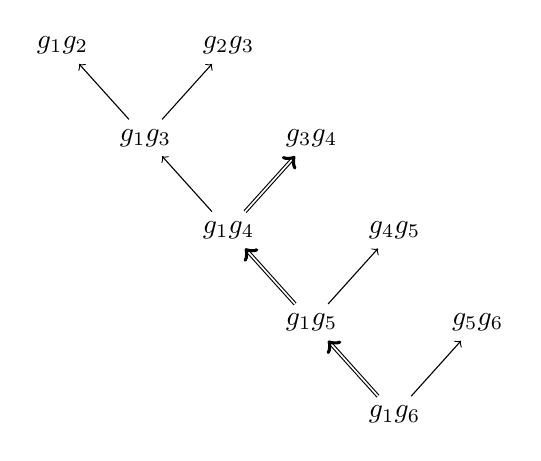
\begin{tikzpicture} [->, baseline=(current bounding box.center)]
    \node {$\subrulep{g_1}{g_6}$} [grow' = up, align=center, anchor=north,
                     sibling distance = 6em, level distance = 4em]
    child {node {$\subrulep{g_1}{g_5}$} edge from parent [double]
      child {node {$\subrulep{g_1}{g_4}$} edge from parent [double]
        child {node {$\subrulep{g_1}{g_3}$}
          child {node {$\subrulep{g_1}{g_2}$}}
          child {node {$\subrulep{g_2}{g_3}$}}
              }
        child {node {$\subrulep{g_3}{g_4}$} edge from parent [double]
              }
            }
      child {node {$\subrulep{g_4}{g_5}$}
            }
          }
    child {node {$\subrulep{g_5}{g_6}$}};
    \end{tikzpicture}
    \hspace*{-2em}$\smash{\transto{0em}}$\hspace*{-2em}
    \begin{tikzpicture} [->, %every edge/.style={draw=none},
                         baseline=(current bounding box.center)]
    \node (g16) {$\nsubrulep{g_1}{g_6}$}
                    [grow' = up, align=center, anchor=north,
                     sibling distance = 6em, level distance = 4em]
    child {node (g15) {$\nsubrulep{g_1}{g_5}$} \efpn
      child {node (g14) {$\nsubrulep{g_1}{g_4}$} \efpn
        child {node (g13) {$\subrulep{g_1}{g_3}$} \efpn
          child {node (g12) {$\subrulep{g_1}{g_2}$}}
          child {node (g11) {$\subrulep{g_2}{g_3}$}}
              }
        child {node (g34) {$\nsubrulep{g_3}{g_4}$} \efpn}
            } 
      child {node (g45) {$\subrulep{g_4}{g_5}$} \efpn}
          }
    child {node (g56) {$\subrulep{g_5}{g_6}$} \efpn};
    \draw (g15) edge [double,->] (g16);
    \draw (g15) edge [dashed,->] (g56);
    \draw (g14) edge [double,->] (g15);
    \draw (g14) edge [dashed,->] (g45);
    \draw (g34) edge [double,->] (g14);
    \draw (g34) edge [dashed,->] (g13);
    \end{tikzpicture}
    \\[1em]
    \phantom{xxxxx}\hfill$\equivto{\sepval}$
    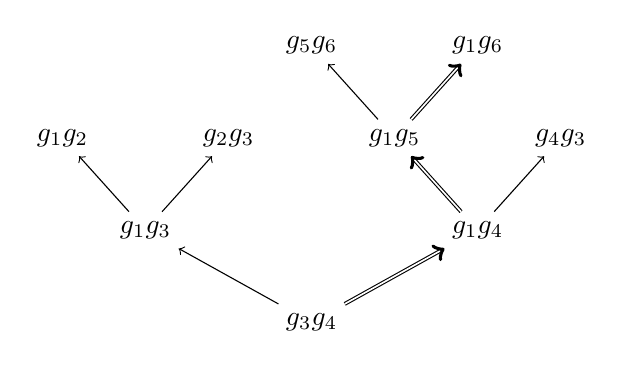
\begin{tikzpicture} [->, baseline=(current bounding box.center),
           level 1/.style={sibling distance=12em},
           level 2/.style={sibling distance=6em},
           level 3/.style={sibling distance=6em}
                        ]
    \node {$\nsubrulep{g_3}{g_4}$} [grow' = up, align=center, anchor=north,
                     level distance = 4em]
    child {node {$\subrulep{g_1}{g_3}$}
      child {node {$\subrulep{g_1}{g_2}$}}
      child {node {$\subrulep{g_2}{g_3}$}}
          }
    child {node {$\nsubrulep{g_1}{g_4}$}
      child {node {$\nsubrulep{g_1}{g_5}$}
        child {node {$\subrulep{g_5}{g_6}$}}
        child {node {$\nsubrulep{g_1}{g_6}$} edge from parent [double]
              }
            edge from parent [double]
            }
      child {node {$\subrulep{g_4}{g_3}$}}
          edge from parent [double]
          };
    \end{tikzpicture}
    \\[1em]
    \phantom{xxxxx}\hfill$\equivto{\sepval}$
   \begin{prooftreem}
     \hypoii{\subrulep{g_1}{g_2}}
            {\subrulep{g_2}{g_3}}
     \inferi{\subrulep{g_1}{g_3}}
     \hypoii{\subrulep{g_5}{g_6}}
            {\nsubrulep{g_1}{g_6}}
     \inferi{\nsubrulep{g_1}{g_5}}
     \hypoi{\subrulep{g_4}{g_3}}
     \inferii{\nsubrulep{g_1}{g_4}}
     \inferii{\nsubrulep{g_3}{g_4}}
    \end{prooftreem}
     \caption{Proof trees for \envref{ex:neginf1}}\label{fig:neginf1}
    \end{figure}
   The first tree, at the top of the figure, represents the proof of
  \nlrightt
   $(\allbinconstrgrsch[\ref{ex:neginf1}]{G}
     \setminus \setbr{\nsubrulep[\gsn]{g_1}{g_6}})
     \union \setbr{\subrulep{g_3}{g_4}} \sentails \subrulep{g_1}{g_6}$
  \newline
 in standard proof-tree format.  Below it, to the left, is this same
tree in vertex-edge format, with the swap path highlighted using
double-line arrows.  This tree is the instantiation, for this example,
of the generic tree of Fig.\ \ref{fig:tocontrap}.  To its right is the
contrapositioning of this tree using fixed vertex positioning,
corresponding to the generic tree of Fig.\ \ref{fig:contrapi}.  The
swap path is again highlighted using double-line arrows, while edges
whose source vertex has been altered as a result of this
transformation are show using dashed lines.  Just below is the same
tree in fixed-edge positioning, corresponding to
Fig.\ \ref{fig:contrapii}, while at the bottom of the figure is the
same result proof in standard inference format.  In all cases, the the
proof rules used have not been identified explicitly, but these are
very easy to determine.
  \end{metalabpara}


 \begin{metalabpara}{myexample}{Example}
    {Inference using a complement-pair rule}\envlabel{ex:neginf2}
   In this example, a proof of unsatisfiability which involves the use
of a complement-pair rule is developed.
   Let $\granschemaname[\ref{ex:neginf2}]{G}$ be an SMAS with
 $\setdef{g_i}{i \in \ccinterval{1}{6}} \subseteq
           \granulesofsch[\ref{ex:neginf2}]{G}$
 and
  \newline
   $\setbr{\subrulep[\gsn]{g_1}{g_2},
          \subrulep[\gsn]{g_2}{g_3},
          \subrulep[\gsn]{g_4}{g_5},
          \subrulep[\gsn]{g_5}{g_6},
          \disjrulep[\gsn]{g_3}{g_6},
          \ndisjrulep[\gsn]{g_1}{g_4}}
   \nlrightt
       \subseteq \allbinconstrgrsch[\ref{ex:neginf2}]{G}$.
    \linebreak
   It will be shown that 
     $\allbinconstrgrsch[\ref{ex:neginf2}]{G}$
 is unsatisfiable, using the proof rules of
$\bininf[\ref{ex:neginf1}]{G}$.
   \begin{figure}[htbp]
    \begin{center}
    \begin{tikzpicture} [->, baseline=(current bounding box.center),
           level 1/.style={sibling distance=12em},
           level 2/.style={sibling distance=12em},
           level 3/.style={sibling distance=6em}
                        ]
    \node {$\false$} [grow' = up, align=center, anchor=north,
                      level distance = 4em]
      child {node {$\disjrulep{g_1}{g_4}$}
        child {node {$\subrulep{g_1}{g_3}$}
          child {node {$\subrulep{g_1}{g_2}$}
                }
          child {node {$\subrulep{g_2}{g_3}$}
                }
              }
        child {node {$\subrulep{g_4}{g_6}$}
          child {node {$\subrulep{g_4}{g_5}$}
                }
          child {node {$\subrulep{g_5}{g_6}$}
                }
              }
        child {node {$\disjrulep{g_3}{g_6}$}
              }
            }
      child {node {$\ndisjrulep{g_1}{g_4}$}
            };
    \end{tikzpicture}
    \\[1em]
    \[
    \begin{prooftreem}
     \hypoii{\subrulep{g_1}{g_2}}
            {\subrulep{g_2}{g_3}}
     \inferi{\subrulep{g_1}{g_3}}
     \hypoii{\subrulep{g_4}{g_5}}
            {\subrulep{g_5}{g_6}}
     \inferi{\subrulep{g_4}{g_6}}
     \hypoi{\disjrulep{g_3}{g_6}}
     \inferiii{\disjrulep{g_1}{g_4}}
     \hypoi{\ndisjrulep{g_1}{g_4}}
     \inferii{\false}
    \end{prooftreem}
    \]
    \end{center}
    \caption{Proof trees for \envref{ex:neginf2}}\label{fig:neginf2}
    \end{figure}
   The strategy is simple.  First, develop a proof that
   $\allbinconstrgrsch[\ref{ex:neginf2}]{G}
         \setminus \setbr{\ndisjrulep{g_1}{g_4}}
         \sentails \disjrulep{g_1}{g_4}$,
  and then apply the complement-pair rule which states that both
elements of the pair
  $\setbr{\disjrulep{g_1}{g_4},\ndisjrulep{g_1}{g_4}}$
 cannot be true.  The associated proof trees, in both vertex-edge
format and traditional logic format, are shown in
Fig.\ \ref{fig:neginf2}.
 \end{metalabpara}


 \begin{metalabpara}{discussion}{}
    {Relationship to RCC5}\envlabel{disc:rcc5}
     Given two granules $g_1, g_2 \in \granulesofsch{G}$, the truth
values of the three sentences $\subrulep{g_1}{g_2}$,
$\subrulep{g_2}{g_1}$, and $\disjrulep{g_1}{g_2}$ together represent
what is known about their relationship.  To formalize this,
% define
% $\truthiii= \setbr{\true,\false,\unknown}$, and
for $\varphi \in \pbinconstrgrsch{G}$, define
   \[
     \gstateof{G}{\varphi} =
        \begin{cases}
          \true ~\text{if}~ \constrgrsch{G} \sentails \varphi, \\
          \false ~\text{if}~ \constrgrsch{G} \sentails \mlnot\varphi, \\
          \unknown ~\text{otherwise},
        \end{cases}
   \]
 and then define the \emph{state vector of} $\grpr{g_1}{g_2}$
\emph{in} $\granschemaname{G}$ to be the triple
 \nlrightt
 $\stateof{G}{g_1}{g_2} =
  \abr{\sstateof{G}{g_1}{g_2},
       \sstateof{G}{g_2}{g_1},
       \dstateof{G}{g_1}{g_2}}$.
  \newline
 Call $\stateof{G}{g_1}{g_2}$ \emph{complete} if no entry has the
value $\unknown$.
   \par
   The \emph{region connection calculus}, or \emph{RCC}, and its
variants, have complete state vectors, rather than individual
predicates, as their starting point.  The papers
 \mycite{RandellCBLR89_kr}, \mycite{RandellCC92_ickrr},
 \mycite{CohnBGG97_geoinf}, \mycite{LiYa03_ai},
 and \mycite{Stell04_amai}
 form a small sample of the vast work in this area.
    The most commonly investigated variant is RCC8, whose associated
state vectors have four entries, since boundaries of regions are also
modelled.  For a comparison to the work of this paper, the more
appropriate variant is RCC5, which focuses on regions without
boundaries, so the state vector has only three entries.  Table
\ref{table:rcc5} shows the state vectors for the version of RCC5
described in \mycite[Table 1]{Stell04_amai}, which is particularly
appropriate for comparison to the granule logic of this paper, since
it supports empty granules, unlike most variants of RCC.\footnote{
     In \mycite[Table 1]{Stell04_amai}, rather than
$\disjrulep{g_1}{g_2}$, a predicate which is best described as
$\subrulep{g_1}{\overline{g_2}}$ is used for the third state
parameter, with $\overline{g_2}$ the complement of $g_2$.  Since
complements are not part of the framework of an SMAS,
$\disjrulep{g_1}{g_2}$ is used instead.  It is easy to verify that the
results are identical.  }
   \begin{table}[htb]
   \begin{center}
   $\begin{array}{*5{|c}|}
     \hline
        & \subrulep{g_1}{g_2}
        & \subrulep{g_2}{g_1}
        & \disjrulep{g_2}{g_1}
        & \text{Symmetric} \\
     \hline\hline
        \rccdc{g_1}{g_2}
                               & \false & \false & \true 
                               & \checkmark \\ \hline
        \rccpo{g_1}{g_2}
                               & \false & \false & \false
                               & \checkmark \\ \hline
        \rcceq{g_1}{g_2}
                               & \true & \true & \false
                               & \checkmark \\ \hline
        \rccpp{g_1}{g_2}
                               & \true & \false & \false
                               &            \\ \hline
        \rccppi{g_1}{g_2}
                               & \false & \true & \false
                               &            \\ \hline
        \rcceqe{g_1}{g_2}
                               & \true & \true & \true
                               & \checkmark \\ \hline
        \rccppe{g_1}{g_2}
                               & \true & \false & \true
                               &            \\ \hline
        \rccppie{g_1}{g_2}
                               & \false & \true & \true
                               &            \\ \hline
   \end{array}$
   \end{center}
   \caption{Predicates of RCC5+}\label{table:rcc5}
   \end{table}
    To avoid any confusion, the variant of RCC described in Table
\ref{table:rcc5} will be called \emph{RCC5+}.
    The predicate names which are used are those which have become
standard in the field.  $\rccdcname$ stands for \emph{disconnected} (\ie,
disjoint), $\rccponame$ for \emph{partial overlap}, $\rcceqname$ for
\emph{equal}, $\rccppname$ for \emph{proper part}, and $\rccppiname$
for \emph{proper part inverse}.  The relations $\rccdcname$,
$\rccponame$, and $\rcceqname$ are \emph{symmetric} in that they are
their own inverses.  On the other hand $\rccppname$ is not symmetric;
hence the need for $\rccppiname$.
    These five relations constitute ordinary RCC5, and are fine as
long as the regions are nonempty.  However, they fail on empty
regions.  The assertions
  $\rcceq{\botgrsch{G}}{\botgrsch{G}}$,
  $\rccpp{\botgrsch{G}}{g_2}$,
 and
  $\rccppi{\botgrsch{G}}{g_2}$
 all fail to hold, the latter two for any $g \in \granulesofschnb{G}$,
counter to the expected meaning of these predicates.
  The solution it to introduce three additional relation names.
  The statements $\rcceq{g_1}{g_2}$, $\rccpp{g_1}{g_2}$, and
$\rccppi{g_1}{g_2}$ cover the cases for which
 $g_1 \not\ideq \botgrsch{G}$, while $\rcceqe{g_1}{g_2}$,
$\rccppe{g_1}{g_2}$, and $\rccppie{g_1}{g_2}$ cover the cases for
which $g_1 \ideq \botgrsch{G}$.
   \par
  A key feature of this framework is that for any pair
$\grpr{g_1}{g_2}$ of granules, $R\grpr{g_1}{g_2}$ holds for exactly
one
 $R \in \setbr{\rccdcname,\rccponame,\rcceqname,\rccppname,
               \rccppiname,\rcceqename,\rccppename,\rccppiename}$.
   This can be seen from the fact that every possible state vector is
represented by one of the predicates.
 This property is sometimes called \emph{JEPD}, short for
\emph{jointly exclusive and pairwise disjoint}.
    \par
  Inference within RCC is often performed via the use of a
\emph{composition table} \mycite{LiYa03_ai}.  Such a table presents,
for
 $R_1, R_2 \in \setbr{\rccdcname,\rccponame,\rcceqname,\rccppname,
               \rccppiname,\rcceqename,\rccppename,\rccppiename}$,
 the relations 
  $R_3 \in \setbr{\rccdcname,\rccponame,\rcceqname,\rccppname,
               \rccppiname,\rcceqename,\rccppename,\rccppiename}$
 for which $R_3 \subseteq R_1 \comp R_2$, with $\comp$ denoting
ordinary relational composition.  Less formally, the table identifies
the relations for which $R_3\grpr{g_1}{g_3}$ could hold, given that
$R_1\grpr{g_1}{g_2}$ and $R_2\grpr{g_2}{g_3}$ hold.  
    \par
   Presenting the entire composition table for RCC5+ is beyond the
scope of this discussion.  However, a simple example of inference is
appropriate, in order to compare RCC5+ to the framework of this paper.
   Let $\granschemaname[\ref{disc:rcc5}]{G}$ have
  $\granulesofschnbnt[\ref{disc:rcc5}]{G} =
         \setbr{g_1,g_2,g_3}$,
 with
 \newline
 \mbox{
  $\constrgrsch{G} =
   \setbr{
    \nsubrulep{g_1}{g_2},
    \nsubrulep{g_2}{g_1},
    \ndisjrulep{g_1}{g_2},
    \subrulep{g_2}{g_3},
    \nsubrulep{g_3}{g_2},
    \ndisjrulep{g_2}{g_3}
         }$.
      }
   It is immediate that these constraints correspond exactly to the
RCC5+ conditions
 \preformat{\linebreak}
  $\setbr{\rccpo{g_1}{g_2}, \rccpp{g_2}{g_3}}$.
   Even without constructing the entire composition table for RCC5+,
it is straightforward to see that $\rccpo{g_1}{g_3}$ and
$\rccpp{g_1}{g_3}$ are the only possibilities for the relationship on
$\grpr{g_1}{g_3}$.  This can be done by looking at a composition table
for RCC8, such as \mycite[Table 2]{LiYa03_ai}, and collapsing
$\rcctppname$ and $\rccntppname$ into $\rccppname$, or just by direct
inspection, drawing a Venn diagram.
    \par
   Now, consider applying the proof rules of
$\bininf[\ref{disc:rcc5}]{G}$.  The only possible deductions are shown
in Fig. \ref{fig:proofsrcc5}.
   \begin{figure}[htb]
    \begin{align*}
     &\begin{prooftreem}
      \hypoii{\subrulep{g_2}{g_3}}
             {\nsubrulep{g_2}{g_1}}
      \inferi{\nsubrulep{g_3}{g_1}}
     \end{prooftreem}
     &&\begin{prooftreem}
      \hypoii{\subrulep{g_2}{g_3}}
             {\ndisjrulep{g_1}{g_2}}
      \inferi{\ndisjrulep{g_1}{g_3}}
     \end{prooftreem}
   \end{align*}
   \caption{Proofs for \envref{disc:rcc5}}\label{fig:proofsrcc5}
   \end{figure}
   For both $\subrulep{g_3}{g_1}$ and $\disjrulep{g_1}{g_3}$ false,
with the truth value of $\subrulep{g_1}{g_3}$ unknown, a check of
Table \ref{table:rcc5} shows that the only possibilities are
$\rccponame\grpr{g_1}{g_3}$ and $\rccppname\grpr{g_1}{g_3}$, in
agreement with the result from a composition table.
    \par
   Whether RCC is preferable to the framework of this paper depends
entirely upon the type of knowledge to be modelled.  If almost all
relationships between granules are known completely, so that one of
the eight predicates of Table \ref{table:rcc5} applies to each pair
$\grpr{g_1}{g_2}$, then RCC will likely be superior.  However, in the
context of substantial incomplete information, RCC will be overwhelmed
by the need for disjunctive representation, rendering the approach of
this paper the preferred one.
 \end{metalabpara}

 \begin{metalabpara}{discussion}{}
    {Relationship to AFDs}\envlabel{disc:afds}
   In \mycite{DeBra87_mfdbs} and \mycite[Sec.\ 5.2]{ParedaensDGV89}, a
framework for dependencies on relational databases which includes both
functional dependencies (FDs) and \emph{afunctional dependencies}
(AFDs) is developed, with a sound and complete inference system.
Since FDs form the original Armstrong context
\mycite{Armstrong74_ifip}, it is worth asking how this work fits into
the framework developed here.
    \par
   AFDs are not true logical negations of FDs.  The relation $R$
satisfies the AFD $\afd{X}{Y}$ if for \textbf{every} tuple $t \in R$,
there is a second tuple $t' \in R$ with $t[X]=t'[X]$ and $t[Y] \neq
t'[Y]$.  On the other hand, the true logical negation of the FD
$\fd{X}{Y}$ has the property that for \textbf{some} tuple $t \in R$,
there is a second tuple $t' \in R$ with $t[X]=t'[X]$ and $t[Y] \neq
t'[Y]$.
   Thus, despite the utility of AFDs, it is not possible to define the
combined inference system for FDs and AFDs by applying the swap
approach of this paper to constraints on FDs.
 \end{metalabpara}


 \begin{metalabpara}{discussion}{}
    {Other contexts}\envlabel{def:otherctxt}
    It should perhaps be mentioned that the techniques of this section
can also be applied to the inference systems $\qbininfpos{G}$ (see
\envref{sum:APinf}) and $\sqbininfpos{G}$ (see
\envref{def:sqbininfpos}), since their underlying frameworks
(consisting of quasi-models and strong quasi-models, respectively),
are easily shown to be Armstrong contexts.  However, this direction
will not be pursued here, since there is no immediate need for the
result.
 \end{metalabpara}

